%----------------------------------------------------------------------------------------
%	PACKAGES AND THEMES
%----------------------------------------------------------------------------------------
\PassOptionsToPackage{table}{xcolor}
\documentclass[aspectratio=169,xcolor=dvipsnames,svgnames,x11names,fleqn]{beamer}
% \documentclass[aspectratio=169,xcolor=dvipsnames,fleqn]{beamer}

\usetheme{RedVelvet}

\usefonttheme[onlymath]{serif}
\newcommand{\showanswers}{yes}


\usepackage{xspace}
\usepackage{amsmath}
\usepackage{amssymb}
\usepackage{amsfonts}
\usepackage{color}
\usepackage{physics}
% \usepackage{mathbb}
\usepackage{rahul_math}
\usepackage{bigints}

\usepackage{graphicx} % Allows including images
\usepackage{booktabs} % Allows the use of \toprule, \midrule and \bottomrule in tables
\usepackage{tikz,pgfplots}

\usepackage{subfigure}
\usetikzlibrary{arrows}
\usepackage{minted}
\definecolor{LightGray}{gray}{0.9}
\definecolor{cream}{rgb}{0.92, 0.9, 0.55}
\definecolor{lightblue}{rgb}{0.68, 0.85, 0.9}


\usepackage{xcolor-material}
\usetikzlibrary{fit}
\usetikzlibrary{matrix}
\tikzset{%
apple/.pic={
    \fill [MaterialBrown] (-1/8,0)  arc (180:120:1 and 3/2) coordinate [pos=3/5] (@)-- ++(1/6,-1/7)  arc (120:180:5/4 and 3/2) -- cycle;
    \fill [MaterialLightGreen500] (0,-9/10)  .. controls ++(180:1/8) and ++(  0:1/4) .. (-1/3,  -1) .. controls ++(180:1/3) and ++(270:1/2) .. (  -1,   0) .. controls ++( 90:1/3) and ++(180:1/3) .. (-1/2, 3/4) .. controls ++(  0:1/8) and ++(135:1/8) .. (   0, 4/7)
    }
    }

\newcommand{\leftdoublequote}{\textcolor{blue}{\scalebox{3}{``}}}

\newcommand{\rightdoublequote}{\textcolor{blue}{\scalebox{3}{''}}}


\usepackage{textcomp}

\usepackage{overpic}

%----------------------------------------------------------------------------------------
%	TITLE PAGE
%----------------------------------------------------------------------------------------

\usepackage{tikz-qtree,tikz-qtree-compat}
\usetikzlibrary{calc}


\title[CPE 486/586: Machine Learning]{CPE 486/586: Machine Learning for Engineers} % The short title appears at the bottom of every slide, the full title is only on the title page
\subtitle{05 Optimization and Gradient Descent}

\author[Rahul Bhadani] {{\Large \textbf{Rahul Bhadani}}}

\institute[UAH] % Your institution as it will appear on the bottom of every slide, maybe shorthand to save space
{
    Electrical \& Computer Engineering,  The University of Alabama in Huntsville
}
\date

% \titlegraphic{
%    \includegraphics[width=0.4\linewidth]{figures/UAH_primary.png}
% }

\begin{document}

%-------------------------------------------------
\begin{frame}
    \titlepage
\end{frame}

%-------------------------------------------------
\begin{frame}{Outline}
    \backgroundtableofcontents
\end{frame}

%%%%%%%%%%%%%%%%%%%%%%%%%%%%%%%%%%%%%%%%%%%%%%%%%%%%%
\begin{sectionframe}{\faGavel}{Optimization}
\end{sectionframe}

\begin{frame}{What is Optimization?}

    \begin{center}
        \begin{enumerate}
            \item Maximizing or minimizing some function relative to some set,
            often representing a range of choices available in a certain situation.
            \item The function
            allows comparison of the different choices for determining which might be ``best".
        \end{enumerate}
    \end{center}
    
\end{frame}

\begin{frame}{A Function with a Minimum}
\begin{center}
\includegraphics[width=0.40\textwidth]{figures/quadratic_surface.pdf}

    This function has a single global minimum.
\end{center}
\end{frame}


\begin{frame}{A Function with a Maximum}
\begin{center}
\includegraphics[width=0.30\textwidth]{figures/maximum_3D.png}

    This function has a single global maximum.
\end{center}
\end{frame}

\begin{frame}
\huge{\centerline{\color{DarkRed}\textbf{How do we find global maximum/minimum}}}
\end{frame}


\begin{frame}{Finding Maxima/Minima of One Variable}
\textbf{A Function of One Variable: $f(x)$}

To find the local maxima and minima of a function $f$ on an interval $[a,b]$:

\begin{itemize}
\item Solve for $f'(x) = 0$ to obtain critical point(s) $c$.
\item Drop from the list any critical points that aren't in the interval $[a,b]$.
\item $x = c$, is a point of local maxima if $f'(c) = 0$, and $f''(c) < 0$. The point at $x= c$ is the local maxima and $f(c)$ is called the \textbf{local maximum} value of $f(x)$.
\item $x = c$ is a point of local minima if $f'(c) = 0$, and $f''(c) > 0$ . The point at $x = c$ is the local minima and $f(c)$ is called the \textbf{local minimum} value of $f(x)$.
\end{itemize}
\end{frame}




\begin{frame}{Example 1}

Find the local maxima and local minima of the function 

%https://www.cuemath.com/calculus/local-maximum-and-minimum/
\begin{multiequation}
f(x) = 2x^3 + 3x^2 -12x + 5
\end{multiequation}

\end{frame}

\begin{frame}{Example 1}

{{\color{gray}{Solution:}}}

\ifthenelse{\equal{\showanswers}{yes}}
{
\begin{columns}
\column{0.5\linewidth}
\begin{multiequation}
\cfrac{\partial f(x)}{\partial x} = 2\cdot 3 x^2 + 3\cdot 2 x - 12 & = 0\\
6x^2 + 6x - 12 & = 0\\
x^2 + x - 2 & = 0\\
x^2 + 2x - x - 2 & = 0\\
x(x+2) - 1(x+2) & = 0\\
(x+2)(x-1) & = 0\\
\Rightarrow  x = -2, x & = 1
\end{multiequation}
\column{0.5\linewidth}
\begin{multiequation}
\cfrac{\partial^2 f(x)}{\partial x^2} & = 12x + 6\\
\cfrac{\partial^2 f(x)}{\partial x^2}\bigg|_{x = -2} & = - 18 < 0\\
\cfrac{\partial^2 f(x)}{\partial x^2}\bigg|_{x = 1} & =  18 > 0
\end{multiequation}
Hence, $x= -2$ for local maximum, and $x= 1$ is for local minimum. $f(-2)$ is local maximum and $f(1)$ is local minimum.
\end{columns}
}

\end{frame}

\begin{frame}{Finding Maxima/Minima of Two Variables}
Consider a function $f(x, y)$ of two variables $x$ and $y$.

If $f$ has a local extremum (or critical point) at $(a, b)$, and if the first order
partial derivatives of $f$ exist there, then

\begin{multiequation}
\cfrac{\partial f}{\partial x}(a, b) = 0 \quad \text{and} \quad   \cfrac{\partial f}{\partial y}(a, b) = 0 \\
or \\
\nabla f(a, b) = \begin{bmatrix}
\cfrac{\partial f}{\partial x}(a, b) &  \cfrac{\partial f}{\partial y}(a, b) 
\end{bmatrix} = \begin{bmatrix}
0 & 0
\end{bmatrix} =  \mathbf{0}
\end{multiequation}

At a critical point, a function
could have a local maximum, or a local minimum,
or neither.

\end{frame}

\begin{frame}{Hessian Function}
If a $f(x, y, z)$ has critical points $(a, b, c)$, then in order to check if it is a maximum, minimum or a saddle point, we need to compute Hessian matrix first.

\begin{columns}
\begin{column}{0.5\linewidth}
    
\begin{equation*}
H = \begin{bmatrix}
\frac{\partial^2 f}{\partial x^2} & \frac{\partial^2 f}{\partial x \partial y} & \frac{\partial^2 f}{\partial x \partial z} \\
\frac{\partial^2 f}{\partial y \partial x} & \frac{\partial^2 f}{\partial y^2} & \frac{\partial^2 f}{\partial y \partial z} \\
\frac{\partial^2 f}{\partial z \partial x} & \frac{\partial^2 f}{\partial z \partial y} & \frac{\partial^2 f}{\partial z^2}
\end{bmatrix}
\end{equation*}
\end{column}
\begin{column}{0.5\linewidth}
    \begin{enumerate}
    \item If all eigenvalues of Hessian function are positive, then $H$ is positive definite, and critical point is local minimum.
    \item If all eigenvalues of Hessian function are negative, then $H$ is positive definite, and critical point is local maximum.
    \item If eigenvalues of Hessian function are  both positive and negative, then critical point is a saddle point.
    \end{enumerate}
\end{column}
\end{columns}


\end{frame}

\begin{frame}{Example 2}
\begin{columns}
\begin{column}{0.5\linewidth}
    Let $z = f (x, y) = x^2 + y^2$. The only critical point is $(0, 0)$. At $(0, 0)$, $f$ has a minimum.
\end{column}
\begin{column}{0.5\linewidth}
    \begin{center}
    \includegraphics[width=0.85\textwidth]{figures/critical_point_ex2.png}
\end{center}
\end{column}
\end{columns}
\end{frame}

\begin{frame}{Example 3}
A cylindrical hot water tank is to have a capacity of 4 $m^3$.
Find the radius and height that would have the least surface area.

{\color{gray}{Solution:}}

\ifthenelse{\equal{\showanswers}{yes}}
{
\begin{columns}
    \column{0.4\linewidth}
    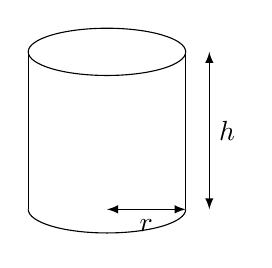
\begin{tikzpicture}[>=latex]

    % Define cylinder dimensions
    \def\radius{1}    % Base radius
    \def\height{2}    % Cylinder height
    \def\perspective{0.3} % Perspective factor for ellipses
    
    % Draw the base (partial front ellipse)
    \draw (-\radius,0) arc (180:360:\radius cm and \perspective cm);
    
    % Draw the back vertical lines
    \draw (-\radius,0) -- (-\radius,\height);
    \draw (\radius,0) -- (\radius,\height);
    
    % Draw the top ellipse
    \draw (0,\height) ellipse (\radius cm and \perspective cm);
    
    % Connect front base to top ellipse (optional, enhances 3D effect)
    %\draw[dashed] (-\radius,0) arc (180:0:\radius cm and \perspective cm);
    
    % Labels
    \draw[<->] (0,0) -- node[below] {$r$} (\radius,0); % Radius label
    \draw[<->] (\radius+0.3,-0.0) -- node[right] {$h$} (\radius+0.3,\height); % Height label
    
    \end{tikzpicture}

    \column{0.4\linewidth}
        \begin{multiequation}
        \pi r^2 h & = 4\\
        h & = \cfrac{4}{\pi r^2}\\
        \end{multiequation}
        Surface Area = $2\pi r^2 + 2\pi r h$

\end{columns}

}

\end{frame}

\begin{frame}{Example 3 Continues ...}

{\color{gray}{Solution:}}

\ifthenelse{\equal{\showanswers}{yes}}
{
\begin{columns}
    \column{0.5\linewidth}
    \begin{multiequation}
    S & = 2\pi r^2 + 8 r^{-1}\\
    \cfrac{\partial S}{\partial r} & = 4\pi r - 8r^{-2}\\
    4\pi r - 8r^{-2} & = 0\\
    r^3 = \cfrac{8}{4\pi}\\
    \Rightarrow r = 0.860
    \end{multiequation}

    \column{0.5\linewidth}
        \begin{multiequation}
        \cfrac{\partial^2 S}{\partial r^2} & = 4\pi + 16r^{-3}\\
        & = 4\pi + \cfrac{16}{(0.860)^3} > 0
        \end{multiequation}
    Hence $r=0.860$ gives minimum surface area, and $S = 2\pi (0.860)^2 + \cfrac{8}{0.860} = 13.949$

\end{columns}


}

\end{frame}


\begin{frame}{Example 4}
Compute local minima/maxima of $f(x, y, z) = x^2 + 2y^2 + 3z^2 - 4x - 6y - 8z + 10$
\end{frame}

\begin{frame}{}

{\color{gray}{Solution:}}

\ifthenelse{\equal{\showanswers}{yes}}
{

\begin{multiequation}
    \nabla f(x, y, z) = \left( \frac{\partial f}{\partial x}, \frac{\partial f}{\partial y}, \frac{\partial f}{\partial z} \right) = \left( 2x - 4, 4y - 6, 6z - 8 \right)
\end{multiequation}
Setting them to $0$, gives $x = 2$, $y = \tfrac{3}{2}$, $z = \tfrac{4}{3}$.

Computing the Hessian matrix:
\begin{multiequation}
    H = \begin{bmatrix}
    2 & 0 & 0\\0 & 4 & 0 \\ 0 & 0 & 6
    \end{bmatrix}
\end{multiequation}
The Hessian matrix's eigen values are $2, 4, 6$ and hence the Hessian matrix is positive definite. Hence, the critical point given by $x = 2$, $y = \tfrac{3}{2}$, $z = \tfrac{4}{3}$ is arg minimum with minimum value at $f(2,\tfrac{3}{2} ,\tfrac{4}{3})$.

}

\end{frame}


%%%%%%%%%%%%%%%%%%%%%%%%%%%%%%%%%%%%%%%%%%%%%%%%%%%%%
\begin{sectionframe}{\faKey}{Constraint Optimization: Lagrange Multiplier}
\end{sectionframe}

\begin{frame}{Lagrange Multiplier}

\begin{center}
The method of Lagrange Multipliers is an excellent technique for finding the global maximum and global minimum values of a function $f(x, y)$ when the values of $x$ and $y$ that need to be considered are subject to some form of constraint, usually expressed as an equation $g(x, y) = 0$.
\end{center}

\end{frame}

\begin{frame}{Problem Formulation}
\textbf{Minimize/Maximize $f(x, y)$}

\vspace{10pt}
subject to

\vspace{10pt}

$g(x, y) = 0$.

\vspace{15pt}

\begin{tblock}{}
In such a case, the optimality occurs when $\nabla f + \lambda \nabla g = 0$.
\end{tblock}
\end{frame}

\begin{frame}{Example 5}
\begin{tblock}{Maximize/Minimize}
Cost function: $f(x, y) = 81x^2 + y^2$, subject to the constraint $4x^2 + y^2 = 0$    
\end{tblock}

\textbf{Solution:}

Lagrange Multiplier is $L(x, y, \lambda) = f(x, y) - \lambda g(x, y)$ where $g(x, y) = 4x^2  + y^2 - 0 = 0$.

\begin{multiequation}
\nabla f = \begin{bmatrix}
    \cfrac{\partial f}{\partial x} & \cfrac{\partial f}{\partial y} 
\end{bmatrix} =  \begin{bmatrix}
    162x & 2y
\end{bmatrix}, \quad \nabla g = \begin{bmatrix}
    \cfrac{\partial g}{\partial x} & \cfrac{\partial g}{\partial y} 
\end{bmatrix}  = \begin{bmatrix}
    8x & 2y
\end{bmatrix}
\end{multiequation}
\end{frame}


\begin{frame}{Example 5 ...}
\begin{multiequation}
\cfrac{\partial f}{\partial x} - \lambda \cfrac{\partial g}{\partial x} & = 0 \Rightarrow 162x  - \lambda 8 x = 0\\
\cfrac{\partial f}{\partial y} - \lambda \cfrac{\partial g}{\partial y} & = 0 \Rightarrow 2y  - \lambda 2y = 0
\end{multiequation}
From the first equation, $8x(21 - \lambda) = 0 \Rightarrow \lambda = 21 $ or $x = 0$.
From the second equation, $2y(1 - \lambda) = 0 \Rightarrow y = 0$ or $\lambda = 1$.

If $x = 0 \Rightarrow 4\cdot 0^2 + y^2 = 9 \Rightarrow y = \pm 3$. Hence the first critical point is $(0, \pm 3)$.

If $y = 0 \Rightarrow 4 x^2 + 0^2 = 9 \Rightarrow x = \pm 3/2$. Hence the second critical point is $(\pm 3/2, 0)$.

$f(0, \pm 3) = 9$ and $f(\pm 3/2, 0 = 729/4 = 182.25$. 


\end{frame}


\begin{frame}{Example 6}

\begin{tblock}{Maximize/Minimize}
Cost function: $f(x, y) = 8x^2 + 2y$, subject to the constraint $x^2 + y^2 = 1$    
\end{tblock}
\end{frame}

\begin{frame}{}

\end{frame}

\begin{frame}{}

\end{frame}

\begin{frame}{Example 7}

\begin{tblock}{Maximize/Minimize}
Cost function: $f(x, y, z) = y^2 - 10 z$, subject to the constraint $x^2 + y^2 + z^2 = 36$    
\end{tblock}

\end{frame}

\begin{frame}{}

\end{frame}

\begin{frame}{}

\end{frame}


\begin{frame}{}

\end{frame}


%%%%%%%%%%%%%%%%%%%%%%%%%%%%%%%%%%%%%%%%%%%%%%%%%%%%%
\begin{sectionframe}{}{Gradient Descent for Optimization}
\end{sectionframe}

\begin{frame}{Algorithmic Approach to Minimizing the Cost Function: Gradient Descent}
The cost function for linear regression with one variable:
\begin{talert}{}
\begin{equation}
    J(w_0, w_1) = \cfrac{1}{2n}\sum_{i=1}^n ( y_i -  w_0 - w_1 x_i )^2
\end{equation}
which is quadratic in $w_0, w_1$. 
\end{talert}

\end{frame}

%------------------------------------------------
\begin{frame}{Gradient Descent}
\begin{center}
        \includegraphics[width=0.40\textwidth]{figures/quadratic_surface.pdf}
        
        This function has a single global minimum.
\end{center}
\end{frame}

%------------------------------------------------
\begin{frame}{Gradient Descent}
\begin{center}
        \includegraphics[width=0.40\textwidth]{figures/quadratic_surface_2.pdf}
        
        This function has two local minima (out of which one is the global minimum).
\end{center}
\end{frame}

%------------------------------------------------
\begin{frame}{Gradient Descent Algorithm}
\begin{talert}{}
We find the minima iteratively:
\begin{equation}
    \begin{aligned}
        w_0 & \leftarrow w_0 - \eta \cfrac{\partial }{\partial w_0}J(w_0, w_1)\\
        w_1 & \leftarrow w_1 - \eta \cfrac{\partial }{\partial w_1}J(w_0, w_1)
    \end{aligned}
\end{equation}
\end{talert}
\end{frame}

\begin{frame}{Gradient Descent Algorithm: Vectorize Form}
\begin{talert}{}
    The partial derivative is the \textbf{gradient} (slope towards the minimum). 
    We iteratively calculate the above equation until $w_0$ and $w_1$ converge. $\eta$ is called the learning rate.  Succinctly, we can write it as 
    \begin{equation}
        \wbf(t+1) \leftarrow \wbf(t) - \eta\nabla J(\wbf(t)) \quad \textrm{where}\quad \nabla J(\wbf) = \begin{bmatrix}
        \cfrac{\partial }{\partial w_0}J(w_0, w_1) \\ \cfrac{\partial }{\partial w_1}J(w_0, w_1)
    \end{bmatrix}
    \end{equation}
    \end{talert}
\end{frame}

%------------------------------------------------
\begin{frame}{Gradient Descent Visualization}
\begin{center}
    \includegraphics[width=0.40\textwidth]{figures/gradient-descent-2D.png}
\end{center}

\end{frame}


%------------------------------------------------
\begin{frame}{Gradient Descent Algorithm: Example 8}

\begin{tblock}{Simple Cost Function}
    \begin{equation}\begin{aligned}
        J(w_1) & = (w_1 - 5)^2 + 10
        \pause\\
        \cfrac{\partial J(w_1)}{\partial w_1} & = 2w_1 - 10
    \end{aligned}
    \end{equation}
    \pause

    We could solve it analytically, but currently, we are interested in solving it numerically using a gradient descent algorithm: $w_1 = w_1 - \eta \cfrac{\partial J(w_1)}{\partial w_1}  $.
    \pause
    
    We start with a few values of $w_1$ and $\eta$.
\end{tblock}
\end{frame}


%------------------------------------------------
\begin{frame}{Batch Gradient Descent}

\begin{itemize}
    \item All training data are taken into account to take a single step.
    \item Take the mean of the gradients of all the training examples to update our parameters.
    \item Requires the entire dataset to be available in the memory.
\end{itemize}
For example, we calculate the gradient of the following:

\begin{equation}
    J(w_0, w_1) = \cfrac{1}{2n}\sum_{i=1}^n ( y_i -  w_0 - w_1 x_i )^2
\end{equation}
\end{frame}


%------------------------------------------------
\begin{frame}{Mini-batch Gradient Descent}

\begin{itemize}
    \item Instead of the entire dataset: we take small random subsets of the training data (mini-batches) at each iteration.
\end{itemize}
We sample a random subset $C_t \subset \{1, 2, \cdots, n\}$, $|C| = b << m$, the batch size, and our update rule is
\begin{equation}
    \wbf(t+1) \leftarrow \wbf(t) -\eta \cfrac{1}{b}\sum_{i \in C_t}\nabla J_i(\wbf(t))
\end{equation}
and full gradient is approximated as
\begin{equation}
    \Ebb\bigg[ \cfrac{1}{b} \sum_{i \in C_t}\nabla J_i(\wbf)\bigg] = \nabla J(\wbf)
\end{equation}
\end{frame}
%------------------------------------------------
\begin{frame}{Stochastic Gradient Descent}

\begin{itemize}
    \item Just use a single training example (or data sample) until a sufficient value is reached for $\wbf$.
    \begin{enumerate}
        \item Take a training data sample, 
        \item Feed to the equation model,
        \item Calculate the gradient,
        \item Update the weights,
        \item Repeated 1-4 for all data samples.
    \end{enumerate}
\end{itemize}

\begin{talert}{}
While the batch gradient descent always converges, it is slow and costly. Stochastic gradient descent is good for the large dataset, makes progress faster, but oscillates in terms converging.
\end{talert}
\end{frame}

%------------------------------------------------
\begin{frame}[containsverbatim]{TensorFlow for Gradient Descent} 

\begin{columns}
    \column{0.5\linewidth}
    \begin{minted}
    [
    framesep=1mm,
    baselinestretch=1.2,
    fontsize=\footnotesize,
    bgcolor=LightJade
    ]
    {python}
import torch
import matplotlib.pyplot as plt

# Define the cost function J(w_1)
def J(w_1):
    return (w_1 - 5)**2 + 10

# Initialize w_1 with requires_grad=True
w_1 = torch.tensor(0.0, requires_grad=True)
# Set up the optimizer
optimizer = torch.optim.SGD([w_1], lr=0.1)
# Store the values of w_1 for plotting
w_1_values = []
    \end{minted}

    \column{0.5\linewidth}

    \begin{minted}
    [
    framesep=1mm,
    baselinestretch=1.2,
    fontsize=\footnotesize,
    bgcolor=sageFuzz
    ]
    {python}
# Perform gradient descent
for i in range(100):
    # Zero the gradients
    optimizer.zero_grad()
    # Compute the loss
    loss = J(w_1)
    # Backward pass (compute gradients)
    loss.backward()
    # Update parameters
    optimizer.step()
    # Store the current value
    w_1_values.append(w_1.item())
plt.plot(w_1_values)
plt.xlabel('Iteration'), plt.ylabel('$w_1$'), plt.show()
    \end{minted}

\end{columns}

\end{frame}

%------------------------------------------------
\begin{frame}[containsverbatim]{Automatic Differentiation} 
\small
\begin{talert}{Automatic Differentiation}
Automatically calculate the derivative of a function by repeatedly applying the chain rule. It can calculate the partial differentiation wrt many inputs. Read more:
\begin{enumerate}
    \item \url{https://www.cs.toronto.edu/~rgrosse/courses/csc321_2018/slides/lec10.pdf}
    \item \url{https://en.wikipedia.org/wiki/Automatic_differentiation}
    \item \url{https://www.tensorflow.org/guide/autodiff}
\end{enumerate}
\end{talert}
\end{frame}


\begin{frame}[containsverbatim]{Automatic Differentiation Example}
    \small
\begin{columns}

\column{0.5\linewidth}
We will construct expression graph of $C(y, wx + b) = y - max(0, wx + b)$ to understand how automatic differentiation works. Automatic differentiation only works with numerical values, hence, let $y = 5,$, $w = 2$, $x=1$, $b=1$.

Our target is to calculate $\cfrac{\partial C}{\partial w_1}$.

\column{0.5\linewidth}
\begin{tikzpicture}[scale=1.0, every node/.style={scale=0.8}]
\node[circle, draw, minimum size=1cm] (minus) at (3,3) {$-$};
\node[circle, draw, minimum size=1cm] (y) at (2,2) {$y$};
\node[circle, draw, minimum size=1cm] (max) at (4,2) {$\max$};
\node[circle, draw, minimum size=1cm] (zero) at (6.5,1) {$0$};
\node[circle, draw, minimum size=1cm] (plus) at (4,1) {$+$};
\node[circle, draw, minimum size=1cm] (b) at (3,0) {$b$};
\node[circle, draw, minimum size=1cm] (times) at (5,0) {$\times$};
\node[circle, draw, minimum size=1cm] (x) at (4,-1) {$x$};
\node[circle, draw, minimum size=1cm] (w) at (6,-1) {$w$};
\node[ellipse, draw, minimum size=1cm] (result) at (3,4.0) {$C$};

\draw[thick] (y) -- (minus);
\draw[thick] (max) -- (minus);
\draw[thick] (max) -- (zero);
\draw[thick] (plus) -- (max);
\draw[thick] (b) -- (plus);
\draw[thick] (plus) -- (times);
\draw[thick] (x) -- (times);
\draw[thick] (w) -- (times);
\draw[thick] (minus) -- (result);
\end{tikzpicture}
\end{columns}
\end{frame}



\begin{frame}[containsverbatim]{Automatic Differentiation Example}\small
\begin{columns}

\column{0.5\linewidth}
    Let: 
    \begin{multiequation}
    w_1 & = w  = 2\quad w_2 = x = 1\\
    w_3 & = b = 1\quad w_4 = y = 5\\
    w_5 & = w_1 w_2 = 2 \quad w_6  = w_3 + w_5 = 3\\
    w_7 & = max(0, w_6) = 3\\
    w_8 & = w_4 - w_7 = 2\\
    C & = w_8 = 2
    \end{multiequation}


\column{0.5\linewidth}
\begin{tikzpicture}[scale=1.0, every node/.style={scale=0.8}]
    \node[circle, draw, minimum size=1cm] (minus) at (3,3) {$-$};
    \node[circle, draw, minimum size=1cm] (y) at (2,2) {$y$};
    \node[circle, draw, minimum size=1cm] (max) at (4,2) {$\max$};
    \node[circle, draw, minimum size=1cm] (zero) at (6.5,1) {$0$};
    \node[circle, draw, minimum size=1cm] (plus) at (4,1) {$+$};
    \node[circle, draw, minimum size=1cm] (b) at (3,0) {$b$};
    \node[circle, draw, minimum size=1cm] (times) at (5,0) {$\times$};
    \node[circle, draw, minimum size=1cm] (x) at (4,-1) {$x$};
    \node[circle, draw, minimum size=1cm] (w) at (6,-1) {$w$};
    \node[ellipse, draw, minimum size=1cm] (result) at (3,4.0) {$C$};

    \draw[thick] (y) -- (minus);
    \draw[thick] (max) -- (minus);
    \draw[thick] (max) -- (zero);
    \draw[thick] (plus) -- (max);
    \draw[thick] (b) -- (plus);
    \draw[thick] (plus) -- (times);
    \draw[thick] (x) -- (times);
    \draw[thick] (w) -- (times);
    \draw[thick] (minus) -- (result);
\end{tikzpicture}
\end{columns}
\end{frame}

\begin{frame}[containsverbatim]{Automatic Differentiation Example}\small
\begin{columns}
    \column{0.5\linewidth}
\begin{multiequation}
\cfrac{\partial w_5}{\partial w_1} & = \cfrac{\partial (w_1\cdot w_2)}{\partial w_1} = w_2\\
\cfrac{\partial w_5}{\partial w_2} & = \cfrac{\partial (w_1\cdot w_2)}{\partial w_2} = w_1\\
\cfrac{\partial w_6}{\partial w_5} & =  \cfrac{\partial (w_5 + w_3)}{\partial w_3} = 1\\
\cfrac{\partial w_7}{\partial w_6} & = \cfrac{\partial max(0, w_6)}{\partial w_6} = \begin{cases} 0, w_6<0\\1 , w_6>0\end{cases}
\end{multiequation}

    \column{0.5\linewidth}
    \begin{multiequation}
    \cfrac{\partial w_8}{\partial w_7} & = \cfrac{\partial (w_4 - w_7)}{\partial w_7} = -1\\
    \cfrac{\partial w_8}{\partial w_4} & = \cfrac{\partial (w_4 - w_7)}{\partial w_4} = 1 \\
    \cfrac{\partial C}{\partial w_8} & = 1
    \end{multiequation}

    Apply chain rule:
    \begin{multiequation}
    \cfrac{\partial C}{\partial w_1} =  \cfrac{\partial C}{\partial w_8} \times \cfrac{\partial w_8}{\partial w_7} \times  \cfrac{\partial w_7}{\partial w_6} \times \cfrac{\partial w_6}{\partial w_5}  \times \cfrac{\partial w_5}{\partial w_1} = ?
    \end{multiequation}
\end{columns}
\end{frame}

\begin{frame}[containsverbatim]{Autograd System} 
\begin{talert}{Autograd System in PyTorch}
PyTorch provides automatic differentiation through its autograd system. It means any operations performed on tensors with \texttt{requires\_grad=True} will automatically compute gradients and build a computational graph dynamically. PyTorch tracks gradients automatically during the forward pass and computes them when \texttt{.backward()} is called.
\end{talert}
\end{frame}

\begin{frame}[containsverbatim]{Example 9}
\begin{minted}
[
framesep=1mm,
baselinestretch=1.2,
fontsize=\normalsize,
bgcolor=white,
]
{python}
import torch
# Initialize x with gradient tracking enabled
x = torch.tensor(3.0, requires_grad=True)
# Compute y = x^3
y = x**3
# Compute gradient dy/dx
y.backward()
# Access the gradient
dy_dx = x.grad
# Convert to numpy if needed
dy_dx.item()  # or dy_dx.numpy() for array format
\end{minted} 
\textbf{What's the output?}
\end{frame}


%------------------------------------------------
\begin{frame}{Some Other Optimizers}
Gradient Descent is one of the many optimizers that can be used to optimize a function and find its minima. Some other commonly popular optimizers are
\begin{enumerate}
\item RMSProp
\item Adagrad (Adaptive Gradient)
\item SGD with Momentum
\item SGD with Nesterov Accelerated Gradient
\item AdaDelta
\item ADAM
\end{enumerate}
\end{frame}

\begin{frame}{RMSProp}
\small
\textbf{RMSProp} (Root Mean Square Propagation) is an adaptive learning rate method that divides the learning rate by an exponentially decaying average of squared gradients.

\begin{itemize}
    \item Update rule:
    \begin{multiequation}
    g_t &= \nabla_\theta J(\theta_t) \\
    v_t &= \beta v_{t-1} + (1 - \beta) g_t^2 \\
    \theta_{t+1} &= \theta_t - \frac{\eta}{\sqrt{v_t} + \epsilon} g_t
    \end{multiequation}
    \item $\eta$: Learning rate
    \item $\beta$: Decay rate (typically 0.9)
    \item $\epsilon$: Small constant for numerical stability
\end{itemize}
\end{frame}

\begin{frame}{Adagrad (Adaptive Gradient)}
\small
\textbf{Adagrad} adapts the learning rate to the parameters, performing smaller updates for frequently occurring features and larger updates for infrequent ones.

\begin{itemize}
    \item Update rule:
    \begin{multiequation}
    g_t &= \nabla_\theta J(\theta_t) \\
    G_t &= G_{t-1} + g_t^2 \\
    \theta_{t+1} &= \theta_t - \frac{\eta}{\sqrt{G_t} + \epsilon} g_t
    \end{multiequation}
    \item $\eta$: Learning rate
    \item $G_t$: Accumulated squared gradients
    \item $\epsilon$: Small constant for numerical stability
\end{itemize}
\end{frame}

\begin{frame}{SGD with Momentum}
\small
\textbf{SGD with Momentum} accelerates gradient descent by adding a fraction of the previous update to the current update.

\begin{itemize}
    \item Update rule:
    \begin{multiequation}
    g_t &= \nabla_\theta J(\theta_t) \\
    v_t &= \gamma v_{t-1} + \eta g_t \\
    \theta_{t+1} &= \theta_t - v_t
    \end{multiequation}
    \item $\eta$: Learning rate
    \item $\gamma$: Momentum term (typically 0.9)
    \item $v_t$: Velocity vector
\end{itemize}
\end{frame}

\begin{frame}{SGD with Nesterov Accelerated Gradient}
\small
\textbf{Nesterov Accelerated Gradient (NAG)} improves momentum by calculating the gradient at the estimated future position.

\begin{itemize}
    \item Update rule:
    \begin{multiequation}
    g_t &= \nabla_\theta J(\theta_t - \gamma v_{t-1}) \\
    v_t &= \gamma v_{t-1} + \eta g_t \\
    \theta_{t+1} &= \theta_t - v_t
\end{multiequation}
    \item $\eta$: Learning rate
    \item $\gamma$: Momentum term (typically 0.9)
    \item $v_t$: Velocity vector
\end{itemize}
\end{frame}

\begin{frame}{AdaDelta}
\small
\textbf{AdaDelta} is an extension of Adagrad that reduces its aggressive, monotonically decreasing learning rate.
\begin{columns}
\column{0.5\linewidth}
\begin{itemize}
    \item Update rule:
    \begin{multiequation}
    g_t &= \nabla_\theta J(\theta_t) \\
    E[g^2]_t &= \rho E[g^2]_{t-1} + (1 - \rho) g_t^2 \\
    \Delta \theta_t &= -\frac{\sqrt{E[\Delta \theta^2]_{t-1} + \epsilon}}{\sqrt{E[g^2]_t + \epsilon}} g_t \\
    E[\Delta \theta^2]_t &= \rho E[\Delta \theta^2]_{t-1} + (1 - \rho) \Delta \theta_t^2 \\
    \theta_{t+1} &= \theta_t + \Delta \theta_t
\end{multiequation}

\end{itemize}

\column{0.5\linewidth}
\begin{itemize}
    \item $\rho$: Decay rate (typically 0.9)
    \item $\epsilon$: Small constant for numerical stability
\end{itemize}
\end{columns}

\end{frame}

\begin{frame}{ADAM (Adaptive Moment Estimation)}
\small
\textbf{ADAM} combines the benefits of RMSProp and Momentum by adapting learning rates and using momentum.

\begin{columns}
\column{0.5\linewidth}
\begin{itemize}
    \item Update rule:
    \begin{multiequation}
    g_t &= \nabla_\theta J(\theta_t) \\
    m_t &= \beta_1 m_{t-1} + (1 - \beta_1) g_t \\
    v_t &= \beta_2 v_{t-1} + (1 - \beta_2) g_t^2 \\
    \hat{m}_t &= \frac{m_t}{1 - \beta_1^t} \\
    \hat{v}_t &= \frac{v_t}{1 - \beta_2^t} \\
    \theta_{t+1} &= \theta_t - \frac{\eta}{\sqrt{\hat{v}_t} + \epsilon} \hat{m}_t
\end{multiequation}
\end{itemize}

\column{0.5\linewidth}
\begin{itemize}
    \item $\eta$: Learning rate
    \item $\beta_1, \beta_2$: Exponential decay rates (typically 0.9 and 0.999)
    \item $\epsilon$: Small constant for numerical stability
\end{itemize}
\end{columns}
\end{frame}



%%%%%%%%%%%%%%%%%%%%%%%%%%%%%%%%%%%%%%%%%%%%%%%%%%%%%
\begin{sectionframe}{\faCrop}{Constraint Optimization with Inequality}
\end{sectionframe}

\begin{frame}{Inequality Constraints}
    
    \Large
    \begin{center}
        $
        \max / \min f(x) 
        $

        subject to 

        $
        g(x) \geq 0
        $
    \end{center}

    Without the constraint, $\cfrac{d f(x^*)}{dx} = 0$.

    When the inequality constraint is added in, either the solution could occur when $g(x^*) = 0$, or $g(x^*) > 0$.
\end{frame}


\begin{frame}{Inequality Constraints with Lagrange Multiplier}

    \begin{center}
    We could still write the Lagrangian:

    \begin{multiequation}
        \Lcal (x,\lambda) & = f(x) + \lambda g(x) \\
        \cfrac{\partial \Lcal}{\partial x}(x^*,\lambda^*)  & =  \cfrac{\partial f}{\partial x}(x^*) + \cfrac{\partial g(x^*)'}{\partial x}\lambda^* = 0\\
        \cfrac{\partial \Lcal}{\partial \lambda}(x^*,\lambda^*) &  = g(x^*) \geq 0\\
        \Rightarrow \lambda^* \geq 0, & \quad \lambda^* \odot  \cfrac{\partial \Lcal}{\partial \lambda} (x^*,\lambda^*)   = \lambda^* \odot g(x^*) = 0\\
            \end{multiequation}

    where $\odot$ is the element-wise product.

These conditions are called \textbf{Karush-Kuhn-Tucker Conditions} (KKT).

    \end{center}

\end{frame}

%------------------------------------------------
\begin{frame}{Karush-Kuhn-Tucker Conditions}
    \begin{itemize}
    \item If we have several equality and inequality constraints, in the following form
    \begin{multiequation}
    \arg\min_{x} f(x), \text{ s.t. } g_i(x) = 0, h_j(x) \leq 0
    \end{multiequation}
    The necessary and sufficient conditions (also known as the KKT conditions) for
    \begin{multiequation}
    &\frac{\partial L(x^*, \lambda^*, \beta^*)}{\partial x} = 0, \hspace{1em}
    \frac{\partial L(x^*, \lambda^*, \beta^*)}{\partial \beta} = 0, \hspace{1em} 
    g_i(x^*) = 0, \hspace{1em}
    h_j(x^*) \leq 0, \\
    &\sum_{j=1}^J \beta_j^* h_j(x^*) = 0, \hspace{1em} 
    \lambda_i, \beta_j \geq 0
    \end{multiequation}
    The last condition is sometimes written in the equivalent form: $\beta_j^* h_j(x^*) = 0$. 
    \end{itemize}
    \end{frame}
    
    
    %------------------------------------------------
    \begin{frame}{The Generalized Lagrangian}
    \begin{tblock}{}
    The generalized Lagrangian function to {\color{MediumRed}minimize} $f(x)$ subject to the equality constraints on $g_i(x)$ and inequality constraints on $h_j(x)$ is given by:  
    \begin{multiequation}
    L(x, \lambda, \beta) = f(x) + \sum_{i=1}^I \lambda_i g_i(x) + \sum_{j=1}^J \beta_j h_j(x)
    \end{multiequation}
    \end{tblock}
    
    \end{frame}
    

% https://home.cc.umanitoba.ca/~lovetrij/cECE7670/2005/Slides/slides7.pdf

% https://pweb.fbe.hku.hk/~pingyu/6066/Slides/LN2_Constrained%20Optimization_slides.pdf

% https://ocw.mit.edu/courses/2-854-introduction-to-manufacturing-systems-fall-2016/6cbf08435a0e531bcfeb396636e216d5_MIT2_854F16_KktExample.pdf

% https://jhc.sjtu.edu.cn/~kuanyang/teaching/MATH3806/notes/lec16.pdf

% https://fedor.iskh.me/backup/econ2125_6012_2024s1/10.constrained.KKT.html

% https://www.stat.cmu.edu/~ryantibs/convexopt-F16/scribes/kkt-scribed.pdf

\begin{frame}{Example 1}

    \begin{columns}
        \column{0.5\linewidth}
        \begin{multiequation}
            \min f(\xbf) =x_1^2 + x_2^2
        \end{multiequation}

        subject to 

        \begin{multiequation}
           x_1 + x_2 & = 1\\
           x_2 \leq \alpha
        \end{multiequation}

        \column{0.5\linewidth}
    \end{columns}


\end{frame}

\begin{frame}{Example 1}
    \begin{columns}

    \column{0.6\textwidth}
    {\color{lightgray}Class Work}
        \column{0.4\textwidth}

    \end{columns}
\end{frame}


\begin{frame}{Example 1}
    \begin{columns}

    \column{0.6\textwidth}
    {\color{lightgray}Class Work}
        \column{0.4\textwidth}

    \end{columns}
\end{frame}


\begin{frame}{Example 1}
    \begin{columns}

    \column{0.6\textwidth}
    {\color{lightgray}Class Work}
        \column{0.4\textwidth}

    \end{columns}
\end{frame}

\begin{frame}{Example 2}

    \begin{columns}
        \column{0.5\linewidth}
        \begin{multiequation}
            \min f(\xbf) = (x_1 - 2)^2 + (x_2 - 1)^2
        \end{multiequation}

        subject to 

        \begin{multiequation}
           h_1(\xbf) & = x_1^2  - x_2 \leq 0\\
           h_2(\xbf) & = x_1  + x_2 - 2 \leq 0
        \end{multiequation}

        \column{0.5\linewidth}
    \end{columns}
\end{frame}


\begin{frame}{Example 2}
    \begin{columns}

    \column{0.6\textwidth}
    {\color{lightgray}Class Work}
        \column{0.4\textwidth}

    \end{columns}
\end{frame}


\begin{frame}{Example 2}
    \begin{columns}

    \column{0.6\textwidth}
    {\color{lightgray}Class Work}
        \column{0.4\textwidth}

    \end{columns}
\end{frame}


\begin{frame}{Example 2}
    \begin{columns}

    \column{0.6\textwidth}
    {\color{lightgray}Class Work}
        \column{0.4\textwidth}

    \end{columns}
\end{frame}

\begin{frame}{Example 2}
    \begin{columns}

    \column{0.6\textwidth}
    {\color{lightgray}Class Work}
        \column{0.4\textwidth}

    \end{columns}
\end{frame}


\begin{frame}{Example 2}
    \begin{columns}

    \column{0.6\textwidth}
    {\color{lightgray}Class Work}
        \column{0.4\textwidth}

    \end{columns}
\end{frame}



\begin{frame}{Further Reading}
\begin{itemize}
\item \url{https://neos-guide.org/guide/algorithms/gradient-projection/}
\item \url{https://www.stat.cmu.edu/~siva/teaching/725/lec6.pdf}
\item \url{https://www.cs.ubc.ca/~schmidtm/Courses/5XX-S20/S5.pdf}
\end{itemize}
\end{frame}

    %------------------------------------------------
    
    \begin{frame}[containsverbatim]{Python Notebook}
    \begin{center}
    \small
    % { \color{Red}{\url{ }}}
    
    \end{center}
    \end{frame}
    
    %------------------------------------------------
    
    \begin{frame}
        \Huge{\centerline{\color{MediumBlue}\textbf{The End}}}
    \end{frame}


\end{document}